\documentclass[11pt,a4paper]{article}


\usepackage[hyperref]{acl}


\usepackage{times}
\usepackage{latexsym}
\usepackage{url}
\usepackage{amsmath}
\usepackage{amssymb}
\usepackage{graphicx}
\usepackage{booktabs}
\usepackage{algorithm}
\usepackage{algorithmic}
\usepackage{caption}
\usepackage{subcaption}
\usepackage{multirow}
\usepackage{array}
\usepackage{placeins}


\newcommand{\E}{\mathbb{E}}
\renewcommand{\P}{\mathbb{P}}
\newcommand{\x}{\mathbf{x}}
\newcommand{\y}{\mathbf{y}}
\newcommand{\Y}{\mathbf{Y}}
\newcommand{\X}{\mathbf{X}}
\newcommand{\D}{\mathcal{D}}
\newcommand{\T}{\mathcal{T}}
\newcommand{\s}{\mathbf{s}}
\renewcommand{\S}{\mathcal{S}}


\usepackage{tabularx}
\newcolumntype{Y}{>{\centering\arraybackslash}X}
\usepackage{mathtools}


\usepackage[dvipsnames]{xcolor}
\usepackage{hyperref}
\hypersetup{
    colorlinks=true,
    linkcolor=blue,
    citecolor=blue,
    urlcolor=blue,
}
\urlstyle{same}


\newcommand*\GitHubLoc{https://github.com/Jeffrey-Ede/ALRC}
\newcommand*\diff{\mathop{}\!\mathrm{d}}
\newcommand*\Diff[1]{\mathop{}\!\mathrm{d^#1}}
\newcommand{\cmark}{\textcolor{ForestGreen}{\checkmark}}
\newcommand{\xmark}{\textcolor{red}{\times}}



%\usepackage[1,2,3,5,6,7]{pagesel} %Discard page 4 as it is blank

% The following packages can be found on http:\\www.ctan.org
%\usepackage{graphics} % for pdf, bitmapped graphics files
%\usepackage{epsfig} % for postscript graphics files
%\usepackage{mathptmx} % assumes new font selection scheme installed
%\usepackage{times} % assumes new font selection scheme installed
%\usepackage{amsmath} % assumes amsmath package installed
%\usepackage{amssymb}  % assumes amsmath package installed

\title{\LARGE \bf
Revisiting Hierarchical Summarization in the Era of LLMs
}

\author{
  Fedor Sobolevsky \And Alexander Kostin \And Konstantin Vorontsov
}

\begin{document}

\maketitle

%%%%%%%%%%%%%%%%%%%%%%%%%%%%%%%%%%%%%%%%%%%%%%%%%%%%%%%%%%%%%%%%%%%%%%%%%%%%%%%%

\begin{abstract}

Hierarchical summarization is a way of organizing information from key points to more specific details. This text summarization method offers a more personalized knowledge acquisition experience, allowing to delve into a topic to any desired extent and only get into more specific details where needed. This method, however, didn't get much attention in scientific literature, possibly due to the lack of quality datasets and proper evaluation metrics. We offer a revision of hierarchical summarization in the era of large language models (LLMs), proposing a novel approach to the task utilizing LLMs and investigating how well such models perform on this task and similar ones. We also propose novel evaluation methods designed specifically for automatic hierarchical summarization evaluation. Furthermore, we provide a new dataset of hierarchical summaries of scientific papers, offering more quality data for the evaluation of hierarchical summarization methods.

\end{abstract}

%%%%%%%%%%%%%%%%%%%%%%%%%%%%%%%%%%%%%%%%%%%%%%%%%%%%%%%%%%%%%%%%%%%%%%%%%%%%%%%%

\section{Introduction}

Modern technology has allowed for a recent surge of the amount of available information in the Internet, and scientific information is no exception. With such amounts of knowledge at our disposal, we need novel ways to organize and summarize it. Recent advances in text summarization, brought about by the rapid development of large language models (LLMs), have made it much easier to process large amounts of information and present it in a simple, user-friendly way. However, traditional text summarization is limited to a fixed summary size, pre-determining the level of detail of the summary. On the contrary, it could be beneficial for the user to have the ability to study a summary with any desired level of detail, diving deeper into more relevant subtopics and covering less relevant ones on a surface level.

Hierarchical summarization, introduced in \cite{christensen2014hierarchical}, aims to solve this exact problem by organizing information hierarchically from key points to more specific details. Their user study confirmed that such a representation of news information is in fact preferred by a large percentage of users. However, this method had got very limited attention and further development, possibly due to the lack of quality text processing methods, limitations of the proposed method, golden-standard datasets and proper evaluation metrics. Nevertheless, we believe that, given the power of modern LLMs, we can revisit this task and offer a novel solution, making hierarchical summarization simple and accessible for a wider range of users. 

In this study, we tackle the problem of hierarchical summarization, given state-of-the-art methods and evaluation tools. Specifically, we make the following contributions:
\begin{enumerate}
    \item We introduce a revised formulation of the hierarchical summarization task.
    \item We describe a novel hierarchical summarization evaluation methodology that takes into account different aspects of hierarchical summary quality.
    \item We introduce a novel dataset of hierarchical summaries of scientific papers, created and verified by experts.
    \item We propose several strategies for automatic hierarchical summary generation using LLMs and extensively evaluate generated summaries.
\end{enumerate}

%%%%%%%%%%%%%%%%%%%%%%%%%%%%%%%%%%%%%%%%%%%%%%%%%%%%%%%%%%%%%%%%%%%%%%%%%%%%%%%%

\section{Related Work}

\paragraph{Text summarization.} While most text summarization methods before the mid-2010s were statistical \cite{gambhir2017recent}, the recent developments in the field are mostly due to the use of machine learning and deep learning techniques \cite{el2021automatic, zhang2025comprehensive}. Particular success in the field has been achieved with the advent of large language models (LLMs), which have become the state-of-the-art tool for text summarization. Furthermore, LLMs have also been found to show promising capabilities in summarization enhancement and evaluation \cite{wu2023large}, \cite{liu2023g}. Some research even suggests, backed by human evaluation, that modern LLMs have reached human-level text summarization capabilities \cite{pu2023summarization}. 

% On the contrary, \cite{zhang2025mixture} note that LLMs cannot explicitly model complex relationships between concepts from different articles, losing information (especially across long contexts), or generating superficial text by listing works without logical connections. To solve these problems, \cite{narayan2021planning} suggest using entity chains, extracting them from text and then adding them to the prompt when generating the final summary. An extensive study on the use of reasoning chains when constructing a prompt for LLMs \cite{wei2023chainofthought} shows the models' intermediate reasoning steps in natural language, which significantly improve performance in various tasks. Another study by \cite{leviathan2025prompt} found that simply repeating the entire prompt twice improves the accuracy of LLM responses without increasing the length of the generated text or increasing latency. 

% \cite{mirasdar2025knowledge} consider the future of text summarization lies in the deep integration of knowledge graphs into LLMs to improve accuracy, validity, and explainability of results. An interesting approach was proposed by \cite{zhang2025mixture}, using an LLM as a flexible extractor of entities and relationships. In the study, this task is performed dynamically, taking into account the context of the entire topic, which allows the graph to be adapted to a specific task.

However, despite the diversity and efficiency of LLM-based summarization methods, generation of structured text representations by LLMs remains understudied. In particular, the ability of LLMs to produce hierarchical summaries has not yet been investigated.


\paragraph{Hierarchical summarization.} The idea of structured text summarization as a more efficient way to summarize large documents appeared in the scientific literature as early as the late 2000s. \cite{yang2008hierarchical}. However, the task was first formalized in \cite{christensen2014hierarchical}. In the initial problem statement, the task of hierarchical text summarization is the task of generating a \textit{hierarchy of summaries} from a collection of documents, in which child summaries expand on the information from the parent summary. The study \cite{christensen2014hierarchical} also proposes a hierarchical summarization method based on hierarchical clustering of sentences followed by summarization of each cluster. The objective function in \cite{christensen2014hierarchical} reflects the salience of the selected sentences, redundancy and coherence (both intra-cluster and parent-child coherence) of the resulting hierarchical summary. 

Although the study shows that hierarchical summaries of news texts are more often preferred by users than traditional approaches, the method is limited to the news domain, as it explicitly incorporates timeline information into the clustering. The idea of hierarchical summarization was since expanded upon only in a small number of studies \cite{litvak2020hierarchical, tauchmann2018beyond}. A dataset containing hierarchical summaries of large, heterogenous document collections has been introduced in \cite{tauchmann2018beyond}.

An alternative form of structured information representation similar to hierarchical summaries is a \textit{mind map} \cite{buzan2006use}. In fact, mind maps, particularly salient-sentence based mind maps (SSM) \cite{wei2019revealing}, can be viewed as a special case of hierarchical summaries, as they also organize textual information into a hierarchy. However, it should be noted that the majority of studies on the topic of mind maps focus on mind maps comprising key snippets or concepts rather than coherent text. 

Nevertheless, in the recent years, a number of studies has also appeared on automatic sentence-based mind map generation \cite{wei2019revealing, hu2021efficient, wang2022multidocument, lu2023weekly, zhang2024coreference}. The methods introduced in these studies are based on generation of a relationship graph for inter-sentence relations (for example, a \textit{coreference graph} \cite{xu2020discourse} as in \cite{zhang2024coreference}), followed by refinement of the graph into a hierarchy. These methods are the most relevant to our study of hierarchical summarization as they as well aim to produce hierarchies of texts based on documents. It is also necessary to mention the recent emergence of numerous commercial AI services for automatic mind map generation. Among such services, one can mention myMap AI\footnote{\texttt{https://www.mymap.ai/mindmap}}, MindMap AI\footnote{\texttt{https://mindmapai.app}}, Mapify\footnote{\texttt{https://mapify.so}} and some others. Despite the prevalence of such services, quality of hierarchical summarization by LLMs remains unbenchmarked.


% \paragraph{Mind maps.} An alternative form of structured information representation similar to hierarchical summaries is a \textit{mind map} \cite{buzan2006use}. In fact, mind maps can be viewed as a type of hierarchical summaries, as they also organize textual information into a hierarchy. Types of mind maps include salient sentence-based mind maps (SSM) and key snippet-based mind maps (KSM) \cite{wei2019revealing}. SSM are more relevant to our study as a form of hierarchical organization of coherent text. However, it should be noted that the majority of studies on the topic of mind maps focus on mind maps comprising key snippets or concepts rather than coherent text.

% Mind maps have been extensively studied as a tool for representing, processing and systematizing knowledge. Numerous studies have investigated the use of mind maps in education, showing that they can in fact improve the quality of infomation retention and understanding in students, including that of scientific information \cite{guerrero2015mind, tungprapa2015effect, rezapour2019mind}. A detailed overview of the use of mind maps in education can be found, for example, in \cite{mitra2023tradition}.

% Most work on automatic mind map generation has focused on concept-based mind maps, utilizing, for example, text mining techniques \cite{abdeen2009direct, elhoseiny2012english2mindmap} as well as machine learning methods, including LLM-based ones \cite{jain2024structsum, vijaykumar2026text}. However, in the recent years, a number of studies has also appeared on automatic sentence-based mind map generation \cite{wei2019revealing, hu2021efficient, wang2022multidocument, lu2023weekly, zhang2024coreference}. The methods introduced in these studies are based on generation of a relationship graph for inter-sentence relations (for example, a \textit{coreference graph} \cite{xu2020discourse} as in \cite{zhang2024coreference}), followed by refinement of the graph into a hierarchy. These methods are the most relevant to our study of hierarchical summarization as they as well aim to produce hierarchies of texts based on documents.

% It is also necessary to mention the recent emergence of numerous commercial AI services for automatic mind map generation. Among such services, one can mention myMap AI\footnote{\texttt{https://www.mymap.ai/mindmap}}, MindMap AI\footnote{\texttt{https://mindmapai.app}}, Mapify\footnote{\texttt{https://mapify.so}} and some others. Despite the prevalence of such services, quality of hierarchical summarization by LLMs remains uninvestigated.


\paragraph{Evaluation metrics.} Most text summarization evaluation methods are based on comparing generated summaries with gold standard summaries created by human experts. Such methods typically use lexical overlap metrics like BLEU \cite{papineni2002bleu}, METEOR \cite{banerjee2005meteor}, and, most popular of them all, ROUGE \cite{lin2004rouge}. These metrics have earned their popularity largely due to their interpretability, however, it has been shown that they poorly model semantic similarity and poorly account for other aspects of summary quality \cite{fabbri2021summeval}.

In the recent years, many LLM-based approaches to summarization evaluation have emerged. Firstly, BERT-like transformer models \cite{devlin2019bert, song2020mpnet, cohan2020specter} have proven to encode text semantics reasonably well, which has made them a promising option for semantic similarity estimation \cite{vrbanec2023comparison, chandrasekaran2021evolution} and, stemming from that, for summarization evaluation \cite{zhang2019bertscore, yuan2021bartscore, laban2022summac}. Furthermore, numerous studies have applied LLMs to automatic scoring of generated summaries without even comparing them with gold standard ones, given the initial text document \cite{chang2023booookscore, wang2023shepherd, gao2023human, wu2023large, liu2023g}. These approaches utilize LLMs' unique abilities to model text semantics and reason, however, it should be noted that there is currently no generally accepted evaluation method among the aforementioned ones, as LLMs are ocasionally prone to errors.

Currently, there exists a variety of metrics for hierarchy comparison. Among the most commonly used metrics are the Robinson-Foulds distance \cite{robinson1981comparison}, the Jaccard index\cite{jaccard1901distribution} and tree edit distance (TED) \cite{zhang1989simple}. Regarding the latter, there exists version of the metric for ordered \cite{zhang1989simple} and unordered \cite{zhang1992editing} trees, algorithms for their efficient computation \cite{pawlik2016tree, schwarz2017new} and a normalization method \cite{li2011metric}, making it a quite versatile metric for tree comparison.

However, when it comes to hierarchical summarization, evaluation metrics are not as abundant, as such metrics have to take into account both semantics and structure of hierarchical summaries. Some studies have employed crowdsourcing for the evaluation of hierarchical summarization and similar tasks, but this approach is costly and lacks reproducibility. Several studies have proposed a metric based on greedy tree alignment and text similarity measurement with ROUGE for mind map comparison \cite{wei2019revealing, zhang2024coreference}. A recent study has proposed a new metric for text tree comparison, text tree edit distance (TTED), based on TED and text similarity measurement using language models \cite{sobolevsky2025text}. It has been proven to be a more reasonable metric for text hierarchies than then previous one, better reflecting significant aspects of text tree difference.


%%%%%%%%%%%%%%%%%%%%%%%%%%%%%%%%%%%%%%%%%%%%%%%%%%%%%%%%%%%%%%%%%%%%%%%%%%%%%%%%

\section{Methodology}

\subsection{Problem Statement}
We'll now proceed with the formulation of the hierarchical summarization problem. A \textit{hierarchical summary}, as in \cite{christensen2014hierarchical}, is a representation of a document or collection of documents in the form of a set of text fragments organized in a hierarchy. Mathematically speaking, a hierarchical summary is an ordered text tree, i.e. a tree (rooted acyclic graph), the vertices of which are ordered and labeled by text fragments. The key feature of a hierarchical summary is that it organizes information in the order from key points to specific details. This means that more general information is located closer to the root of the hierarchy than details. Moreover, child nodes of a given node of the tree expand on the information in the parent node. This principle is key for hierarchical summaries, as it gives the user the option to delve into more details on any specific topic from the document or, alternatively, cover it on a surface level. Formally, the user can \textit{expand} the summary in an arbitrary way, i.\,e. hide or show child nodes of any node in the hierarchy depending on their desired level of detail.

The loss function in \cite{christensen2014hierarchical} optimizes for \textit{salience}, \textit{non-redundancy} and \textit{coherence}, both parent-to-child and intra-cluster. We reformulate these criteria into the following requirements for hierarchical summaries:
\begin{enumerate}
    \item \textbf{Completeness:} a hierarchical summary, expanded to an arbitrary depth, is a complete summary of the source document. This particularly means that the most general information from the source document should be located in the highest levels of the hierarchy. This way, when reading the summary on a surface level, the user should still be able to get a brief understanding of the whole document without leaving out any key aspects.
    \item \textbf{Conciseness:} a hierarchical summary, expanded to an arbitrary depth, should be concise, i.\,e. it should present information from the source document in as brief of a way as possible without losing any relevant information. This entails that specific details that are unnecessary for general understanding of the source document should be moved lower into the hierarchy. This requirement also implies that a hierarchical summary should be non-redundant, just like a regular text summary.
    \item \textbf{Coherence:} a hierarchical summary, expanded to an arbitrary depth, should be coherent when read in depth-first order. This requirement stems from the natural order in which users read hierarchies. It entails that the following node pairs should be read coherently:
    \begin{itemize}
        \item parent node~--- first child node;
        \item neighboring sibling nodes;
        \item last node of subtree~--- root of next subtree.
    \end{itemize}
    Fig. \ref{fig:reading_order} illustrates this requirement for clarity.
\end{enumerate}

\begin{figure}
    \centering
    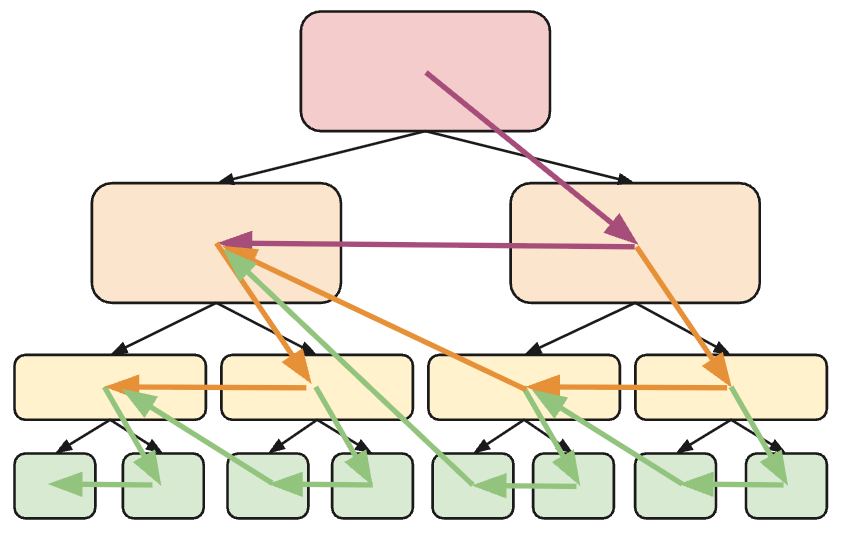
\includegraphics[width=0.8\linewidth]{img/reading_order.png}
    \caption{The order in which a hierarchical summary should be read coherently. Arrows mark node pairs that should be coherent.}
    \label{fig:reading_order}
\end{figure}


\subsection{Method}

\textcolor{Red}{TODO}

%%%%%%%%%%%%%%%%%%%%%%%%%%%%%%%%%%%%%%%%%%%%%%%%%%%%%%%%%%%%%%%%%%%%%%%%%%%%%%%%

\section{Experimental Setup}

\subsection{Models}

\textcolor{Red}{TODO}

\subsection{Dataset}

\textcolor{Red}{TODO}

\subsection{Metrics}

To extensively evaluate generated hierarchical summaries, we use a variety of metrics covering different aspects of summary quality. As a hierarchical summary is a text tree, i.\,e. it combines the features of a tree and a text summary, it is necessary to evaluate both the structure and the textual contents of a hierarchical summary to assess its quality. This can be done via comparison with golden-standard summaries or using reference-free quality metrics. The goal for comparative metrics is to achieve lower difference between generated and reference summaries that between different references. For reference-free metrics, the goal is to achieve comparable or better scores than reference summaries.

To assess overall difference between hierarchical summaries, we use \textbf{TTED}, proposed in \cite{sobolevsky2025text}. It is defined as tree edit distance between summaries where the costs of edit operations are determined by semantic distance between texts, estimated by a predefined language encoder model. To get normalized values of TTED for summaries of different sizes, we use the normalization procedure described in \cite{li2011metric}:
\begin{equation}
    \tilde{d}(T_1, T_2) = \frac{2\cdot d(T_1, T_2)}{\alpha(|T_1| + |T_2|) + d(T_1, T_2)},
\end{equation}
where $\alpha$ is the maximum insertion/deletion cost for both summaries $T_1$ and $T_2$.

We also use a modification of TTED that aims to assess structural difference between trees, \textbf{structural TTED (STTED)}. It is defined as ordinary tree edit distance between text trees with costs of all operations equal to 1, except for update operations for semantically equivalent nodes. Semantic equivalence is again determined by a predefined language encoder with a similarity threshold taken from \cite{vrbanec2023comparison}.

We also introduce several metrics aiming to reflect different components of TTED. Particularly, we take the optimal edits from TTED and measure:
\begin{enumerate}
    \item The cost of \textbf{insertions};
    \item The cost of \textbf{deletions};
    \item The cost of \textbf{structural edits} (insertions and deletions);
    \item The cost of \textbf{semantic edits} (node updates);
    \item The \textbf{average semantic distance} between nodes in semantic edits;
    \item The \textbf{average depth difference} between nodes in semantic edits;
    \item The \textbf{percentage of equivalent node pairs} in semantic edits.
\end{enumerate}
This suite of metrics is used to investigate the different aspects in which summaries differ independently rather than using an aggregated difference estimate.

We can also measure similarity between the textual contents of hierarchical summaries. To do this, we convert hierarchical summaries to linear text by reading them in DFS order. To measure text similarity, we use \textbf{ROUGE-1, -2} and \textbf{-L} for lexical similarity and BERTScore for semantic similarity.

Next, we use a number of reference-free metrics to assess the quality of generated and reference summaries independently. Since such metrics are defined only for linear text summaries, we, again, convert summaries to linear text. To evaluate summary consistency, we use \textbf{SummaC} \cite{laban2022summac} (particularly its two variants, SummaC$_\text{Conv}$ and SummaC$_\text{ZS}$). Also, we use \textbf{G-Eval} \cite{liu2023g} to assess fluency, coherence, consistency and relevance of summaries via LLM-as-a-judge.

Finally, we calculate each metric for summaries, expanded to different depths. Specifically, for each summary $T$ and each depth $k\leq\text{depth(T)}$, we calculate each metric for $T$, expanded to depth $k$. This way, we can assess the quality of hierarchical summaries at different levels of abstraction. 

%%%%%%%%%%%%%%%%%%%%%%%%%%%%%%%%%%%%%%%%%%%%%%%%%%%%%%%%%%%%%%%%%%%%%%%%%%%%%%%%

\section{Results}

\textcolor{Red}{TODO}

%%%%%%%%%%%%%%%%%%%%%%%%%%%%%%%%%%%%%%%%%%%%%%%%%%%%%%%%%%%%%%%%%%%%%%%%%%%%%%%%

\section{Discussion}

\textcolor{Red}{TODO}

%%%%%%%%%%%%%%%%%%%%%%%%%%%%%%%%%%%%%%%%%%%%%%%%%%%%%%%%%%%%%%%%%%%%%%%%%%%%%%%%

\section{Conclusion}

\textcolor{Red}{TODO}

%%%%%%%%%%%%%%%%%%%%%%%%%%%%%%%%%%%%%%%%%%%%%%%%%%%%%%%%%%%%%%%%%%%%%%%%%%%%%%%%


\bibliographystyle{acl_natbib}
\bibliography{bibliography}

\clearpage

\end{document}